\documentclass[sigconf]{acmart}

\usepackage{booktabs} % For formal tables
\usepackage{graphicx}  
\usepackage{listings}
%\usepackage{pxfonts}
%\usepackage{color}
\usepackage{xcolor}
\usepackage{lmodern}
\usepackage[T1]{fontenc}
\usepackage{xparse}% http://ctan.org/pkg/xparse
 \usepackage{tikz}
\usepackage{pgfplots}
\NewDocumentCommand{\Log}{o}{%
  \IfNoValueTF{#1}{}{{}^{#1}\!}\log}%

\settopmatter{printacmref=false} % Removes citation information below abstract
\renewcommand\footnotetextcopyrightpermission[1]{} % removes footnote with conference information in first column
\pagestyle{plain} % removes running headers

% Copyright
%\setcopyright{none}
%\setcopyright{acmcopyright}
%\setcopyright{acmlicensed}
%\setcopyright{rightsretained}
%\setcopyright{usgov}
%\setcopyright{usgovmixed}
%\setcopyright{cagov}
%\setcopyright{cagovmixed}

% DOI
%\acmDOI{xx.xxx/xxx_x}

% ISBN
%\acmISBN{xxx-xxxx-xx-xxx/xx/xx}

%\copyrightyear{2017} 
%\acmYear{2017} 
%\setcopyright{rightsretained} 
%\acmConference{IWOCL '17}{May 16-18, 2017}{Toronto, Canada}
%\acmDOI{http://dx.doi.org/10.1145/3078155.3078183}
%\acmISBN{978-1-4503-5214-7/17/05}

\makeatletter
\newcommand\BeraMonottfamily{%
	\def\fvm@Scale{0.75}
	\fontfamily{fvm}\selectfont
}
\makeatother

\definecolor{sh_comment}{rgb}{0.12, 0.38, 0.18 }
\definecolor{sh_keyword}{rgb}{0.37, 0.08, 0.25}
\definecolor{sh_string}{rgb}{0.06, 0.50, 0.68}

\lstset { %
	language={[11]C++},
	%basicstyle=\small,
	%stringstyle=\ttfamily,
	basicstyle= \BeraMonottfamily,
	keywordstyle=\bfseries,
	frame = single,
    stringstyle=\color{sh_string},
    keywordstyle = \color{sh_keyword}\bfseries,
	commentstyle=\color{sh_comment}\itshape,
    lineskip=-0.3em,
	morekeywords={
		vxCreateGenericNode,
		vxSetParameterByIndex,
		vxSetKernelAttribute,
		vxProcessGraph,
		vxAddParameterToKernel,
		clCreateProgramWithSource,
		vxFinalizeKernel,
		clCreateKernel,
		clEnqueueNDRangeKernel,
		clSetKernelArgs,
	},
	escapeinside=!!
}

\definecolor{bostonuniversityred}{rgb}{0.8, 0.0, 0.0}
\definecolor{goldenbrown}{rgb}{0.6, 0.4, 0.08}
\newcommand\setc[1]{\hspace{-1ex}\textcolor{blue}{\bf\BeraMonottfamily{#1}}}
\newcommand\setv[1]{\hspace{-1ex}\textcolor{bostonuniversityred}{\bf\BeraMonottfamily{#1}}}
\newcommand\setd[1]{\hspace{-1ex}\textcolor{goldenbrown}{\bf\BeraMonottfamily{#1}}}


\begin{document}
\title{FFT Based Convolution}
%\titlenote{Produces the permission block, and
%  copyright information}
%\subtitle{Extended Abstract}
%\subtitlenote{The full version of the author's guide is available as
%  \texttt{acmart.pdf} document}

\author{Vikram Chandrashekar}
\affiliation{%
	\institution{Virginia Tech}
}
\email{vikramc@vt.edu}
\author{Ariel Bernal}
\affiliation{%
  \institution{Intel Corporation}
}
\email{ariel.j.bernal@intel.com}

% The default list of authors is too long for headers}
\renewcommand{\shortauthors}{A.Bernal}


\begin{abstract}
Training deep learning models is taking increasingly longer time as the models grow bigger and the sizes of the datasets keep increasing. Convolution operation accounts for most of the time required for training a network. Also, inference applications are increasingly requiring real time response. A faster convolution can make both training and inference faster by reducing the computation time, as convolution operation constitutes more than 70\% of operations in deep learning networks. In this paper, we try to optimize convolution operation using FFT. We compare off the shelf FFT libraries with a new FFT implementation designed with convolution operation as the end goal, and we study the impact on convolution operations.
\end{abstract}


% We no longer use \terms command
%\terms{Theory}

\keywords{Fft, Convolution, Deep Learning}

\maketitle

\section{Introduction}

Deep learning applications are achieving state of the art results in many domains, overtaking human levels of performance. These range from the traditional applications of image recognition and object classification to the strategy based games such as chess and go. A quick look at the network evolution over the last couple of years reveals that networks are getting deeper in terms of number of layers [1]. As a consequence, the training time has gone up from days to couple of weeks even when running the training on multiple nodes using sophisticated graphics cards in parallel configuration. For example, in the latest state-of-the-art model [2] at the time this paper is written needs 500 GPUs across 4 days.

Inference stage of deep learning applications such as object recognition or image segmentation need real time response for use in applications such as self-driving cars. The more commercialized applications like the filters on Snapchat or Instagram apps are mobile based augmented reality applications which needs to process the image in real time and in a computationally constrained environment such as mobile phone. Even after upgrading the processors to the latest generation, the throughput (number of images processed per second) does not seem to be increasing as much as expected. This is because the models are becoming bigger and complex to extract more intricate features.

Out of the many components that we can try to optimize to make the deep learning models run faster, convolution seems to be the most promising. This is because more than 70\% of the time  running a forward pass and a backward pass of a deep learning model is spent in convolution operation at various layers of the network. So an efficient convolution operation has the potential to improve the performance of a network considerably.

In this paper, we first briefly introduce the different approaches for convolution currently being used in various frameworks and illustrate their advantages and disadvantages.

This is followed by explanation of the actual process of how to use FFT to get convolution operation. The specific approach used in this project for parallelizing the implementation of FFT is discussed followed by the optimizations we have incorporated into this FFT keeping convolution as end goal. Finally, we compare the throughput performance of our approach versus a benchmark and investigate the reasons for the observed results.

\section{CONVOLUTION APPROACHES}
\subsection{Spatial Domain Convolution}

Spatial domain convolution is the method we use to calculate the convolution operation by hand. We multiply elements at corresponding positions of image and kernel and then add these partial products together to get a single number which is the result of this convolution. Fig.\ref{SpatialConvolutionIllustration} illustrates this operation. The kernel is then moved by stride units across the image in both horizontal and vertical direction and we repeat the convolution operation. After sliding the kernel over the entire image, we obtain the result for the full image. 

\begin{figure}[h] 
	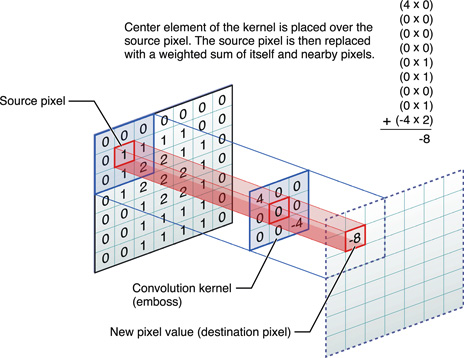
\includegraphics[width=8cm]{images/SpatialConvolution.png}
	\caption {Spatial Convolution Illustration}
	\label{SpatialConvolutionIllustration}
\end{figure}

The advantage of this operation is its simplicity. There are no overhead operations in terms of re-arranging the matrix data and it involves direct matrix multiplication. This approach works for image sizes which are smaller, otherwise the overhead of re-arranging the matrix which other convolution methods require outweighs the actual computation for small matrices. While this approach is simple to implement and understand, it does not necessarily parallelize well on a GPU.

\subsection{GEMM (GEneral Matrix Multiply)}
GEMM uses highly optimized matrix multiplication libraries such as BLAS (Basic Linear Algebra Subprograms) at the back end to do the actual computations. However, to use matrix multiplications for convolution we need to rearrange the matrix wherein we divide the $n$ dimensional image into smaller 
blocks. Each of these sub blocks in the image is then serialized into a one dimensional row. Similarly, the sub blocks of other matrix are drawn out into columns. These are multiplied using library routines. The results will need to be re-arranged back into appropriate dimensions again based on the number of filters. Fig. 2 illustrates these operations. 

GEMM is widely used for matrices of intermediate dimension. In other words, it is suitable for larger matrices so that the overhead of re-arranging the data is small compared to the number of actual computations. The disadvantage of this approach is the higher memory requirement. The re-arranged matrix consists of many copies of the elements from the original matrix since we need to copy a row/column of data which will be shared across different strides of the kernel into a separate row/column.


\begin{figure}[h] 
	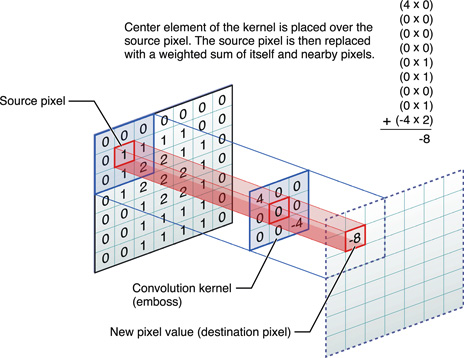
\includegraphics[width=8cm]{images/SpatialConvolution.png}
	\caption {GEMM Convolution Illustration \\ The green matrix is formed by stretching out the sub blocks of image into rows. The orange block is formed by stretching out the kernel sub blocks into columns. These are multiplied and then reshaped into appropriate dimensions}
	\label{GEMMConvolutionIllustration}
\end{figure}

\subsection{FFT (Fast Fourier Transform)}
The main idea in using FFT to compute convolution is that convolution in the time domain becomes multiplication in the frequency domain. Multiplications have a lesser amount  of computations over convolutions, and we are utilizing this principle to optimize the convolution by converting them into frequency domain representation. This is illustrated by the equation in Fig.3 which represents the relationship between the time domain and frequency domain counterparts. 
The FFT method also involves re-arranging the input image and kernel into a specific format before actually computing the FFT. This basically involves padding the matrix to make it suitable for circular convolution which is what an FFT does. The FFT of an image and kernel are multiplied element-wise along the depth. The elements are summed up across the depth and then the inverse FFT is taken over the 2-D matrix. A crop of this 
result is the actual convolution result. Fig. 4 illustrates these pre-processing steps.

The advantage of using FFT is that it is a well-studied technique since the early ages of signal processing and there are highly optimized implementations for parallel computing. Also, FFT gives the best advantage when the image and kernel size is larger. This is because FFT method does not need to move over the image in strides, but a single FFT gives the convolution result for the whole image. The only downside is the overhead of re-arranging the matrix for FFT and the actual process of computing the FFT.

There are other advantages of choosing an FFT based convolution implementation as listed below:
\begin{enumerate}
\item Convolution in the time domain becomes multiplication in the frequency domain. This reduces the sheer number of add-multiplies. [11] describes the theoretical computations of both direct method and the FFT method, and it shows that as the size of the input increases, FFT based method tends to outperform the direct method by a large margin.
\item During inference runs where we care about throughput (processing more images per unit time), instead of storing the learned kernel weights, we can store the FFT of the learned kernel and hence can significantly reduce the overhead of FFT computation. We eliminate the need to compute FFT over kernels and now we only need to compute FFT of image and then inverse FFT of the results.
\item Since the input to a convolution is an image, such real valued signals have "nice" properties which render themselves to highly optimized computations. These properties will be explained in the implementation part of the paper.
\end{enumerate}

\section{FFT Based Implementations}
There are many implementations of FFT available as libraries. clFFT [3], FFTW [4] are few popular, generic examples. While using such off-the shelf generic FFT libraries can greatly reduce the development cycle, these libraries are not developed keeping convolution as the end goal,  so a lot of optimizations which can be implemented for convolution as end goal will not be available in these. Additionally, these libraries need to support a wide range of input sizes. However, with regard to convolution for deep learning applications, the number of possible input matrix sizes we need to handle is way less. Having this knowledge about the end application, we can use it in the implementation for optimizations and hence achieve better throughputs. While a custom FFT for convolution will not be suitable for generic applications, it will be highly efficient as it is tailored for the application.

There is also a recent implementation of FFT using cuda [12] for GPU based systems, called as fbFFT. fbFFT paper proposes an implementation of FFT optimized specifically using cuda. There are two points on which our approach differs fundamentally from this paper although the end goals of both papers are the same, that is to optimize convolution:

\begin{enumerate}
\item The fbFFT is based on cuda which is specific to GPUs from a specific hardware vendor and is closed source. Any changes including development to this environment is tightly controlled as it is closed source and hence not available for public contribution.
\item While discrete GPUs seem to be the workhorse for many deep learning models running on cloud servers, there are many emerging use cases which run on a processor,  an FPGA or heterogeneous compute platforms.	
\end{enumerate}

Because of the above points, we chose OPENCL [5] as the language of source for our implementation. While OPENCL is open source and the enhancements are driven by the community, it also supports many platforms. It can run on anything from a CPU to a GPU to an FPGA. These aligned closely with our goals for the project and hence we made the choice of using OPENCL. So the broad goal of this project was to develop an optimized parallel implementation of FFT keeping convolution as the end goal to support heterogeneous compute platforms.

\section{Split Stream FFT}
The algorithm we chose for our parallel implementation is based on a paper called split stream FFT [6]. The split stream algorithm was chosen for its following merits:
\begin{enumerate}
\item Conventional FFTs need strided memory access between intermediate stages of computation. This is because of the butterfly structure of the FFT algorithm. Whereas split stream algorithm re-arranges the input data initially before the computation and eliminates the need for strided memory access.
\item The algorithm is suitable for parallel implementation with less dependencies and bottlenecks compared to serial implementations of FFT.
\end{enumerate}
Fig.5 shows the block diagram for the split stream FFT. First we will look at how to do FFT along a single dimension and then we will extend this to a 2D FFT. A row of data is considered a work group, which means the threads within this work group can share data across each other using a shared memory and also the steps can be synchronized across threads.
\begin{enumerate}
\item Bit reversal: The left most block is the first stage. The data needs to be re-arranged in bit-reversed order initially to avoid the strided reads in later stages. The positions of bit reversed indices are pre-computed and stored in main memory. The data is read with this indexing so that when they are stored in registers of a thread they are in the bit-reversed order. This helps in saving time as compared to the method of reading in the whole row and then trying to swap the elements into their correct position in place.
\item Work item: Every two consecutive elements are handled by a single thread and this forms a work item. So for a row of size $n$, there are $\frac{n}{2}$ work items and up to $\frac{n}{2}$ threads. This is because the mapping is not one to one between a work item and a thread, as the compute units use SIMD (Single Instruction Multiple Data) to do vector operations. A single thread can, in theory, do 32 length vector operations (SIMD32) on the machine that we are testing on [13]. In practice, of course, it is vectorized as much as is allowed by other dependent resource such as registers and barriers.
\item Twiddle factors: Computing FFT needs complex exponentials often called the twiddle factors. Since computing these on the fly can take time and also as they are reused for every row, it makes sense to compute them pre-hand and store in shared memory. Each work item reads only the twiddle factor which it needs for computing its elements from the common memory space. 
\item Each work item does following operations: it adds the two elements it is working on and stores the result in a shared memory space of the workgroup. Similarly, it subtracts the two elements and multiplies the difference with the twiddle factor and stores the result again to the shared memory.
\item We wait until all the work items have finished step (4) before the next stage. This is achieved using a barrier. After that, the output computed by the threads at the end of stage (4) forms input for the next stage and we repeat steps (2) through (4) for $x$ iterations where $ x = \log _2 n $, $n$ is row size.	
\end{enumerate}

The implementation uses decimation in frequency approach. The above yields 1D-FFT for a row of data. We launch as many work groups as there are number of rows, so we get one dimensional FFT for each row, but we need 2D-FFT for our convolution operation. To get this, we transpose the 1D-FFT result and then take row-wise 1D-FFT again over this and do a transpose of the result. This method works because FFT is separable linearly along its dimensions. Doing single dimension FFT twice saves computations as compared to doing a complex two dimensional FFT in one go. One optimization here is that we can eliminate the second transpose. This is because the FFT results of image and kernel are multiplied elementwise, and then we take inverse FFT to get the time domain values. Hence the two transpose operations cancel each other. Another optimization is computing the first transpose. Usually transpose operation does not render itself well for parallel computations, therefore there are methods which do tiled transpose, wherein they read a small square tile and write it out transposed. This is to coalesce the memory accesses. In our approach, since the data was already in the registers after computation we could do a scattered write to the transposed positions. Hence thereby avoiding reading the data again from main memory.

\section{Results}
We chose clFFT as the benchmark to compare against our implementation. The results of split stream FFT were validated against an online implementation of FFT to verify the functional correctness of the algorithm. After that we compared the run time of our FFT for one dimensional inputs of different sizes which are relevant to convolution operation. Fig. \ref{fft_1d} shows this plot, where input size is on the horizontal dimension and the speedup of our FFT versus clFFT is plotted in the vertical axis. A speedup of 1 means that both implementations are taking the same time. Whereas a speedup of more than one implies our FFT is faster. As seen in the plot, our FFT outperforms clFFT by at least 1.5x across the input sizes. For some input sizes it outperforms by up to 3x as seen from the plot, but it is an improvement overall in the input range of interest.

\begin{figure}[h] 
\centering
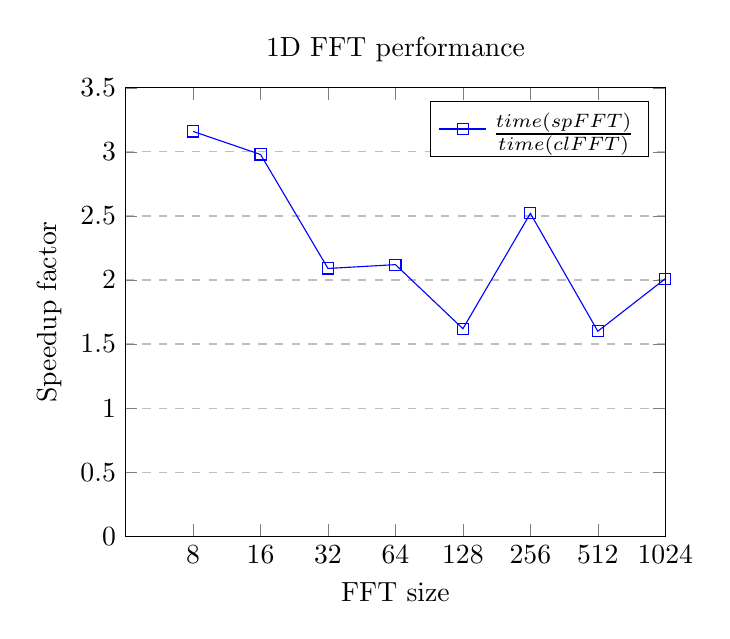
\begin{tikzpicture}
\begin{axis}[
    title={1D FFT performance},
    xlabel={FFT size},
    ylabel={Speedup factor},
    xmin=0, xmax=1024,
    ymin=0, ymax=3.5,
    symbolic x coords={0, 8, 16, 32, 64, 128, 256, 512, 1024},
    xtick=data,
    ytick={0, 0.5, 1, 1.5, 2, 2.5, 3, 3.5},
    legend pos=north east,
    ymajorgrids=true,
    grid style=dashed,
]
 
\addplot[
    color=blue,
    mark=square,
    ]
    coordinates {
    (8,3.16)(16, 2.98)(32, 2.09)(64, 2.12)(128, 1.62)(256, 2.52)(512, 1.6)(1024, 2.01)
    };
    \legend{$\frac{time(spFFT)}{time(clFFT)}$}
 
\end{axis}
\end{tikzpicture}
	\caption {Plot showing 1D-FFT throughput ratio comparison with varying input sizes}
	\label{fft_1d}
\end{figure}

Next in Fig. \ref{fft_2d} we plot the performance for 2D-FFT. It seems that the 2D-FFT is performing better than benchmark for inputs of smaller size, but does not scale well for larger size inputs. The observed results were confirmed over multiple runs. 

\begin{figure}[h] 
\centering
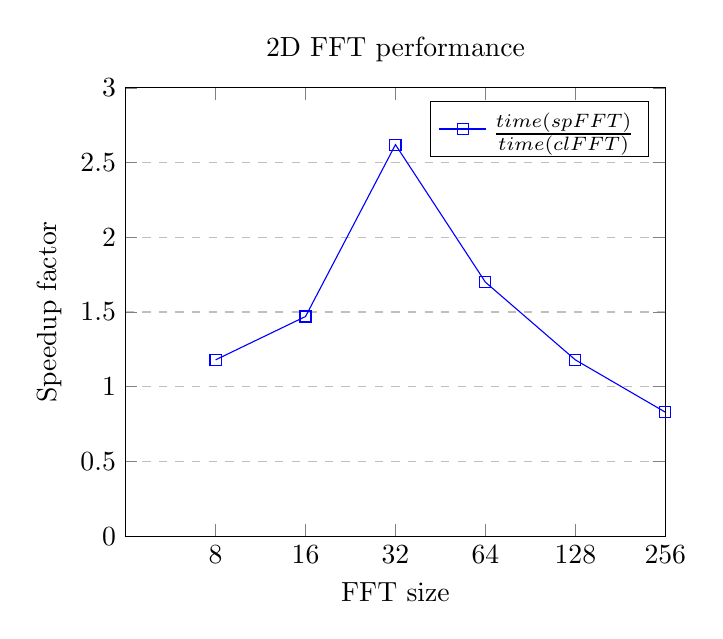
\begin{tikzpicture}
\begin{axis}[
    title={2\-D FFT performance},
    xlabel={FFT size},
    ylabel={Speedup factor},
    xmin=0, xmax=256,
    ymin=0, ymax=3,
    symbolic x coords={0, 8, 16, 32, 64, 128, 256},
    xtick=data,
    ytick={0, 0.5, 1, 1.5, 2, 2.5, 3},
    legend pos=north east,
    ymajorgrids=true,
    grid style=dashed,
]
 
\addplot[
    color=blue,
    mark=square,
    ]
    coordinates {
    (8,1.18)(16, 1.47)(32, 2.62)(64, 1.7)(128, 1.18)(256, 0.83)
    };
    \legend{$\frac{time(spFFT)}{time(clFFT)}$}
 
\end{axis}
\end{tikzpicture}
	\caption {Plot showing 2D-FFT throughput ratio comparison with varying input sizes}
	\label{fft_2d}
\end{figure}

\section{Analysis}
One dimensional FFT outperforms significantly better than benchmark. But the same scaling was not seen in two dimensional FFT. Analysis of the kernel logs did not seem to point anything wrong with the implementation, but analysis of the benchmark revealed that the algorithm switches between two different radix decimations. In our algorithm, we always use radix 2 and we need logarithm (to base 2) number of iterations to compute the output FFT. However, if we use a higher radix, like radix 4 the number of iterations needed to compute the output reduces. According to [7] radix 4 algorithm provides a saving of 15\% over radix 2, so it seems the benchmark algorithm switching over to radix 4 when the input is more than a certain threshold starts to outperform at larger input sizes. From this point onwards the performance improvement we obtained from all the optimizations starts to wane compared with the radix 4 algorithm. 

There is also documented usage of mixed radix where in bigger radix is used in initial stages to bring down the computations and when the inputs are under a certain range we revert back to smaller radix. This may also yield performance improvements.


\section{Optimizations}
Our implementations make use of many of the nice properties of FFT for real valued signals. One of them is the Hermitian property : FFT of a real valued signal is a complex conjugate signal. This allows us to combine two rows into a single row by placing one row as the real part and the other row as the imaginary part. Then we compute single FFT of this complex signal and extract the FFT of the individual rows. Also, because of Hermitian property, when we take 2D FFT of a real valued signal we can crop half of the matrix after the 1D FFT, as the data will be complex conjugate and then compute FFT over half the matrix. The FFT so obtained can be restored to full length post computation.

\section{Future Work}
As identified in the previous section, we can try to use radix 4 to reduce the computations and hence to increase the throughput. Another idea is that we can, in theory, avoid scrambling the input data if we do decimation in time for forward FFT and then do decimation in frequency for inverse FFT.

\section{Conclusion}
In this project we implemented a new FFT keeping the end goal of convolution and which can operate on heterogeneous compute platforms. The new FFT was shown to be outperforming the benchmark for one dimensional case and performed quite well for initial range of inputs for two dimensional case. The possible choices for improving the performance further were identified.


\let\thefootnote\relax\footnote{Intel and the Intel logo are trademarks of Intel Corporation or its subsidiaries in the U.S. and/or other countries.*Other names and brands may be claimed as the property of others. OpenCL and the OpenCL logo are trademarks of Apple Inc. used by permission by Khronos.}  
	
\bibliographystyle{ACM-Reference-Format}
\bibliography{sigproc} 

\end{document}
